\chapter{Types and Expressions}
\label{typeexpr}

In the following sections \emph{Ident} refers to a variable identifier of the graph model language (see \ref{modelbb}) or the rule set language (see \ref{rulebb}). By analogy \emph{TypeIdent} is a identifier of a type.

\section{Built-In Types}
\label{builtin}
Besides user-defined node types, edge types and enum types, GrGen supports the built-in primitive types in table \ref{builtintypes}:
\begin{table}[htbp]
\begin{tabularx}{\linewidth}{|l|X|}\hline
	\texttt{boolean} & Covers the values \texttt{true} and \texttt{false}. \\
	\texttt{int} & A 32-bit signed integer, in two's complement representation. \\
	\texttt{float}, \texttt{double} & A floating-point number in IEEE 754 format with single precision or double precision respectively. \\
	\texttt{String} & A sequence of digits, letters, underscores and white spaces. Strings are of arbitrary length and may be enclosed by double quotes. If the string contains white spaces, double quotes are mandatory.\\ \hline
\end{tabularx}
\caption{\GrG\ built-in types}
\label{builtintypes}
\end{table}

\section{Expressions}
\label{expressions}
\begin{rail}
  Expression: BoolExpr | IntExpr | FloatExpr | StringExpr | PrimaryExpr ;  
  BoolExpr: ((() | '(' 'boolean' ')') (() | '!') PrimaryExpr) | (BoolExpr '?' BoolExpr ':' BoolExpr) | (BoolExpr ([1] doubleampersand | [2] '||') BoolExpr) | (Expression CompareOperator Expression) | (TypeExpr CompareOperator TypeExpr);
\end{rail}
As in C, \texttt{!} negates a boolean, \texttt{\&\&} is a logical AND and \texttt{||} is a logical OR. The order of precedence is \texttt{!}, \texttt{\&\&}, \texttt{||}. The \texttt{?} operator is a simple if-then-else: if the first \emph{BoolExpr} is evaluated to \texttt{true}, the operator returns the second \emph{BoolExpr}, otherwise it returns the third \emph{BoolExpr}.\\
\emph{CompareOperator} is one of the following operators:
\[ \texttt{<} \;\;\;\;\; \texttt{<=} \;\;\;\;\; \texttt{==} \;\;\;\;\; \texttt{!=} \;\;\;\;\; \texttt{>=} \;\;\;\;\; \texttt{>} \]
Table \ref{compandtypes} describes the semantics of compare operators on type expressions.
\begin{table}[htbp]
\label{compandtypes} 
  \begin{tabularx}{\linewidth}{|l|X|} \hline
    \texttt{A == B} & True, iff $A$ and $B$ are identical. Different types in a type hierarchy are \emph{not} identical. \\
    \texttt{A != B} & True, iff the $A$ and $B$ are not identical. \\
    \texttt{A < B} & True, iff $A$ is a supertype of $B$, but $A$ and $B$ are not identical. \\
    \texttt{A > B} & True, iff $A$ is a subtype of $B$, but $A$ and $B$ are not identical. \\
    \texttt{A <= B} & True, iff $A$ is a supertype of $B$ or $A$ and $B$ are identical. \\
    \texttt{A >= B} & True, iff $A$ is a subtype of $B$ or $A$ and $B$ are identical. \\ \hline
  \end{tabularx}
\caption{Compare operators on type expressions}
\end{table}

\begin{rail}
  IntExpr: ((() | '(' 'int' ')') (() | '+' | '-' | tilde) PrimaryExpr) | (BoolExpr '?' IntExpr ':' IntExpr) | (IntExpr BinaryOperator IntExpr);
\end{rail}
Boolean and enum types (and technically integer types) can be converted to \texttt{int} by using the \texttt{(int)} construct. The $\sim$ operator is a binary NOT. That means every bit of an integer value will be flipped. The \texttt{?} operator is a simple if-then-else: if the \emph{BoolExpr} is evaluated to \texttt{true}, the operator returns the first \emph{IntExpr}, otherwise it returns the second \emph{IntExpr}.\\ 
\emph{BinaryOperator} is one of the operators in table \ref{tabbinops}:
\begin{table}[htbp] 
  \centering
  %\begin{tabularx}{0.45\linewidth}{|ll|} \hline
  \begin{tabular}[c]{|lp{0.6\linewidth}|} \hline
    \begin{tabular}[c]{l} \texttt{|} \\ \texttt{\^} \\ \texttt{\&} \end{tabular} & \begin{tabular}[c]{l} Binary OR, XOR and binary AND \end{tabular} \\ \hline
    \begin{tabular}[c]{l} \texttt{\mbox{<}\mbox{<}} \\ \texttt{\mbox{>}\mbox{>}} \\ \texttt{\mbox{>}\mbox{>}\mbox{>}} \end{tabular} & \begin{tabular}[c]{l} Bitwise shift left, bitwise shift right and \\ bitwise shift right with respect to sign \end{tabular}\\ \hline
    \begin{tabular}[c]{l} \texttt{+} \\ \texttt{-} \end{tabular} & \begin{tabular}[c]{l} Addition and subtraction \end{tabular}\\ \hline
    \begin{tabular}[c]{l} \texttt{*} \\ \texttt{/} \\ \texttt{\%} \end{tabular} & \begin{tabular}[c]{l}Multiplication, integer division \\ and modulo \end{tabular} \\ \hline
  \end{tabular}
  \caption{Binary integer operators, in ascending order of precedence}
  \label{tabbinops}
\end{table}

\begin{rail}  
  FloatExpr: ((() | '(' ('float' | 'double') ')') (() | '+' | '-') PrimaryExpr) | (BoolExpr '?' FloatExpr ':' FloatExpr) | (FloatExpr ('+' | '-' | '*' | '/') FloatExpr);
\end{rail} 
Type conversion by \texttt{(float)} and \texttt{(double)} is possible between \texttt{float} and \texttt{double} only. The \texttt{?} operator is a simple if-then-else: if the \emph{BoolExpr} is evaluated to \texttt{true}, the operator returns the first \emph{FloatExpr}, otherwise it returns the second \emph{FloatExpr}.

\begin{rail}
  StringExpr: PrimaryExpr | StringExpr '+' StringExpr;
\end{rail}
The operator \texttt{+} concatenates two strings.

\begin{rail} 
  PrimaryExpr: '(' Expression ')' | Ident (() | ('.' Ident +)) | (EnumType '::' Ident) | TypeIdent | 'typeof' '(' Ident ')' | Constant;
  Constant: Number | HexNumber | QuotedText | 'true' | 'false';
\end{rail}

\section{Type Expressions}
\label{typeexpressions}

\begin{rail}
  TypeExpr: TypeIdent | 'typeof' '(' Ident ')' ;
\end{rail}
A type expression identifies a type (and -- in terms of matching -- also its subtypes). A type expression is either a type identifier itself or the type of a variable.\\
{\small \textbf{Example:}\\
The following rule will add a reverse edge to an one-way street.}
\begin{grgen}
rule oneway {
    pattern{
        a:Node -x:street-> y:Node;
        negative{
            y -:typeof(x)-> a;
        }
    } 
    replace{
      a -x-> y;
      y -:typeof(x)-> a;
    }
}
\end{grgen}

\begin{rail}
  TypeConstraint: backslash '(' (TypeExpr + '+')  ')' ; 
\end{rail}
A type constraint is used to exclude parts of the type hierarchy. The operator \texttt{+} is used to identify a unification of types.\\
{\small \textbf{Example:}}\\
\begin{tabularx}{\linewidth}{c|X}
  \begin{tabular}[c]{c}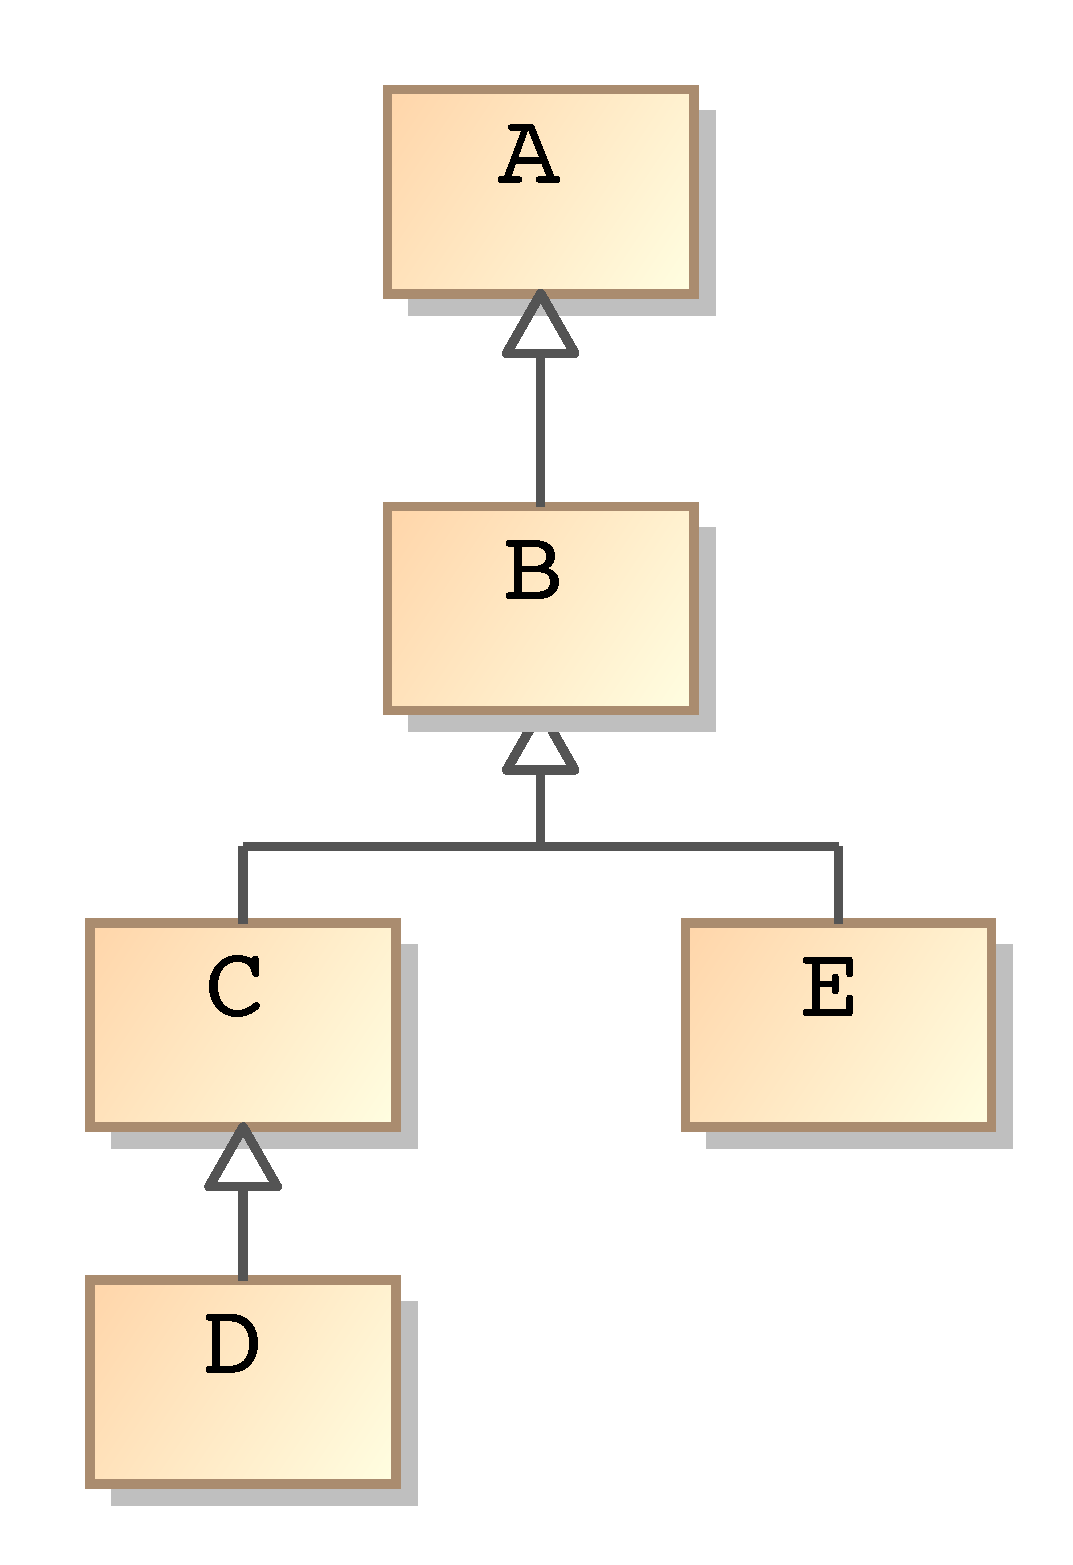
\includegraphics[width=0.35\linewidth]{fig/hierarchy}\end{tabular} & {\small The expression \texttt{A\char"5C (C+E)} applied to the type hierarchy on the left site covers $A$ and $B$.}\\
\end{tabularx}

\section{Annotations}
\label{annotations}

Identifier definitions can be annotated by pragmas. Annotations are key-value pairs.
\begin{rail}
  IdentDecl: Ident (() | '[' (Ident '=' Constant + ',') ']');
\end{rail}
Although you can use any identifier between the brackets, only the identifier \texttt{prio} has an effect so far.
\begin{table}[htbp]
\begin{tabularx}{\linewidth}{|lllX|} \hline
  \textbf{Keyword} & \textbf{Type} & \textbf{Applies to} & \textbf{Meaning} \\ \hline
  \texttt{prio} & int & node, edge & Changes the ranking of a graph element for search plans. The default is \texttt{prio}=1000. Graph elements with high values are likely to appear prior to graph elements with low values in search plans. {\small \textbf{Example:} We search the pattern \texttt{v:NodeTypeA -e:EdgeType-> w:NodeTypeB}. We have a host graph with about 100 nodes of \texttt{NodeTypeA}, 1,000 nodes of \texttt{NodeTypeB} and 10,000 edges of \texttt{EdgeType}. Furthermore we know that between each pair of \texttt{NodeTypeA} and \texttt{NodeTypeB} there exists at most one edge of \texttt{EdgeType}. Wen can use this information to improve the initial search plan, if we adjust the pattern like \texttt{v[prio=10000]:NodeTypeA -e[prio=5000]:EdgeType-> w:NodeTypeB}}. \\ \hline
\end{tabularx}
\caption{Annotations}
\label{tabannotations}
\end{table}


